For all parts of this question I have assumed $T = 300 \textrm{ K}$ and have used values appropriate for silicon.
\subsection*{a)}
	\begin{figure}[htbp!]
		%	\centering
		\flushright
		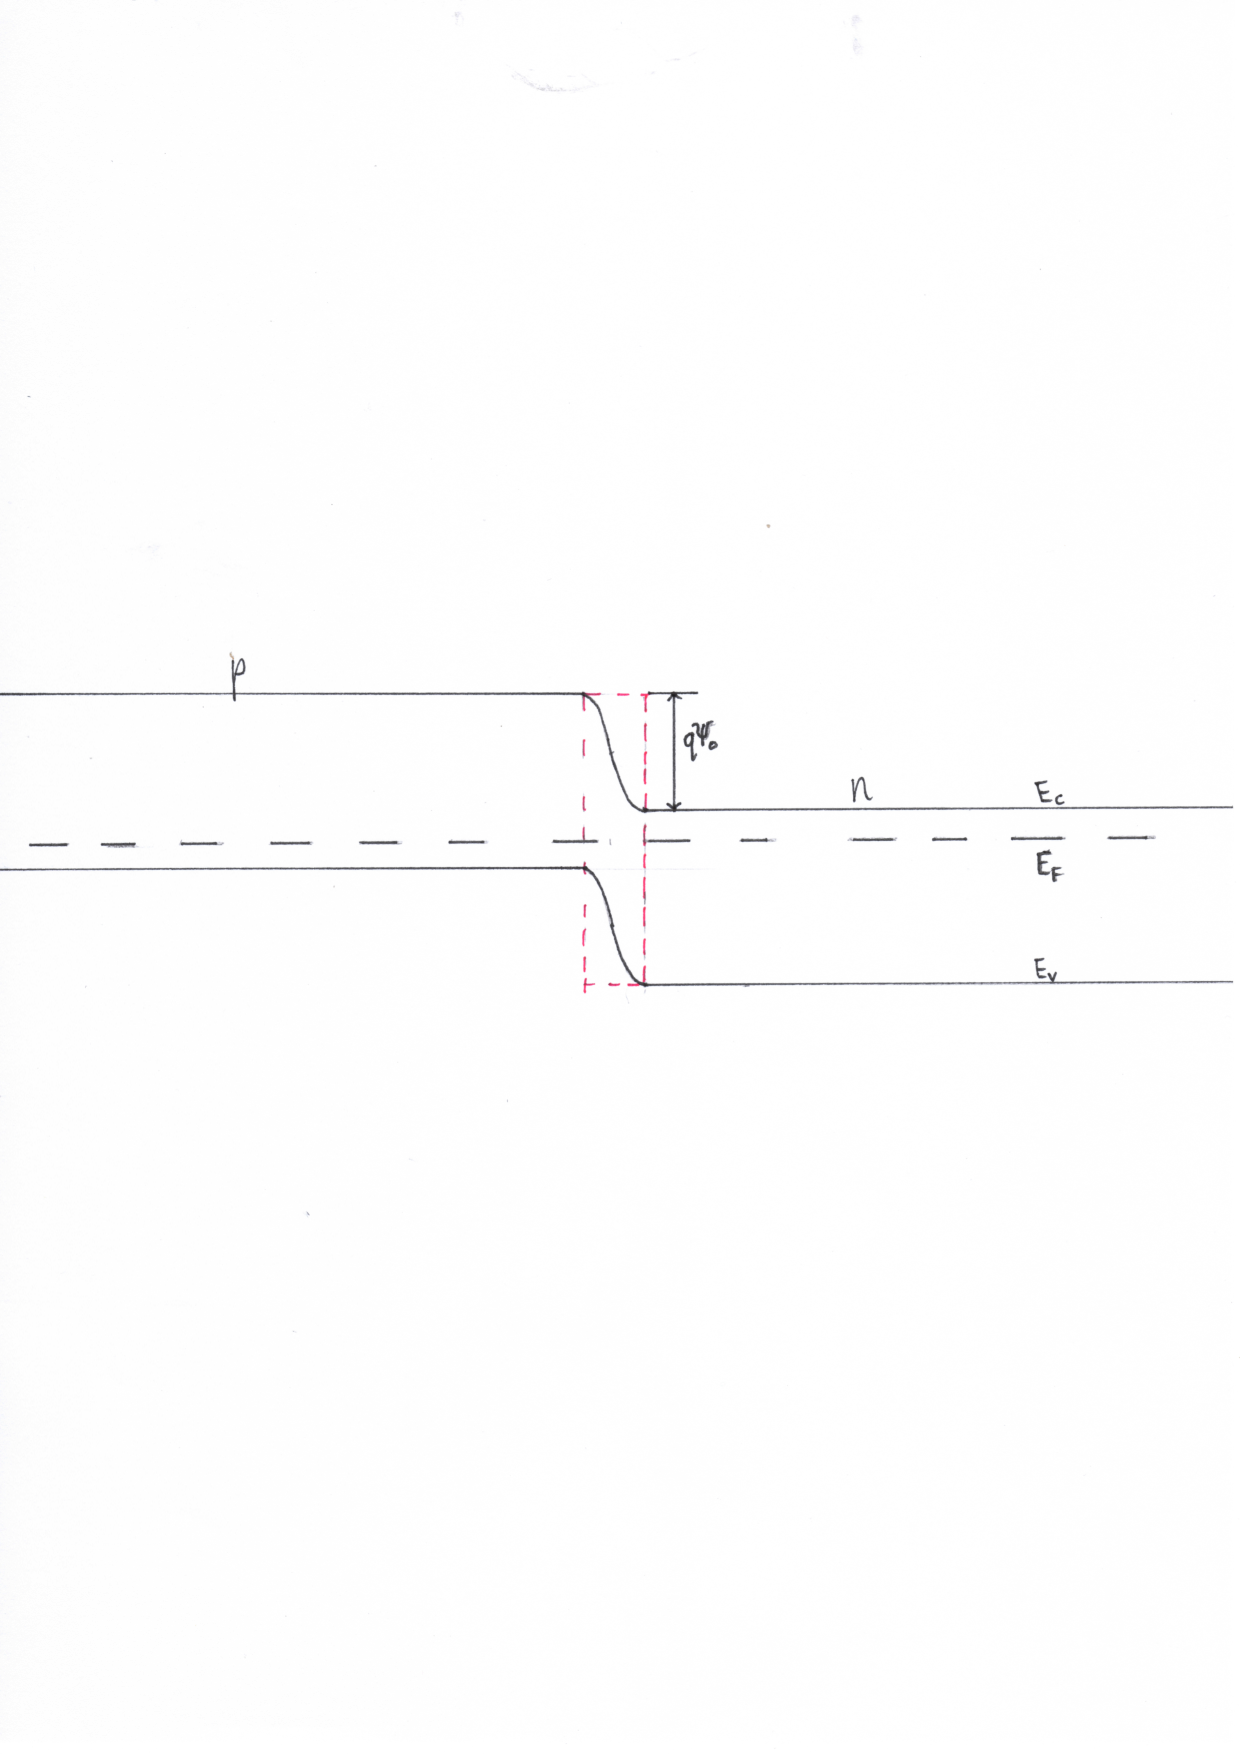
\includegraphics[trim={3.5cm 12.5cm 2.5cm 11cm},clip]{./img/2a}
		\caption{Energy diagram of a pn junction.}
	\end{figure}
	\[
	\begin{aligned}
		q \psi_0 &= E_C(p) - E_C(n) \\
			   &= (E_F + E_G - E_1) - (E_F + E_2) \\
			   &= E_G - E_1 - E_2 \\
			   &= 1.12 \textrm{ eV} - k T \ln \left( \frac{N_V N_C}{N_A N_D} \right) \\
			\psi_0  &=	1.12 \textrm{ V} - 0.147 \textrm{ V} \\
			   &= 0.973 \textrm{ V}	   
	\end{aligned}
	\]
\subsection*{b)}
\subsection*{c)}
	
